% ------------------------------------------------------------
\section{Calendar Week}
% ------------------------------------------------------------
% --------------------------------------------------- Slide --
\subsection{CW 09}
% ------------------------------------------------------------
\begin{frame}
  \frametitle{Review CW 09}
	\begin{itemize}
		\item All APDL Script tutorials/exercises regarding remodelling algorithm provided by the University of Ulm were tested. Where possible, results were checked against analytical calculations. \textcolor{green}{Done}
		\item Backup of files in the MHH PC where organized. "Readme" file under \path{\ZPR\2_Forschung\Bereiche\WPL\FEM\BLuna\6_Ansys} now contains a detailed description of how to restore the files. Also the overview of the Ansys files created is available in the the same folder. \textcolor{green}{Done}
	\end{itemize}
\end{frame}

\begin{frame}
  \frametitle{Review CW 09 - First Remodeling Simulations}
	\begin{figure}
		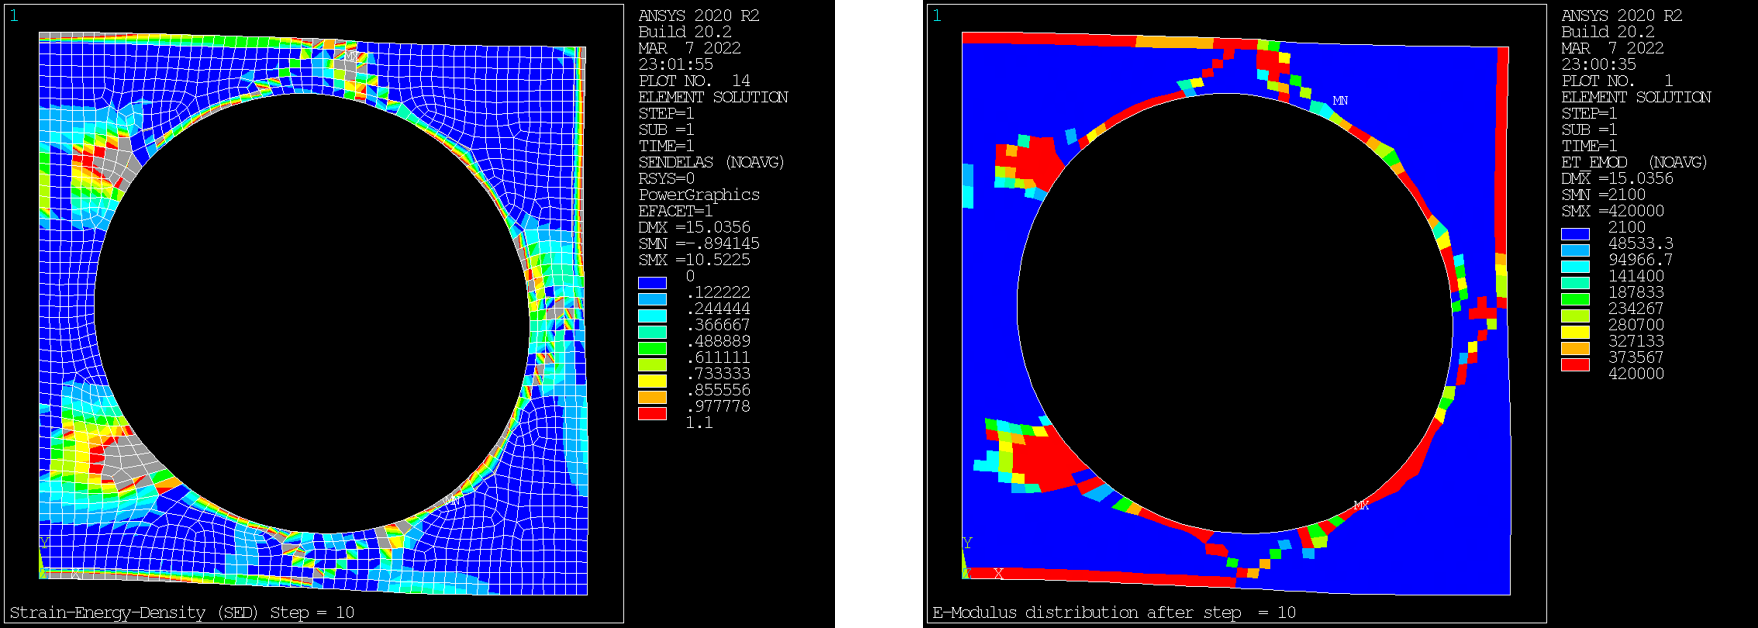
\includegraphics[width=0.9\textwidth]{pictures/2022_CW09}
	\end{figure}
	\centering Plate fixed on the left edge and with downward force on the right edge.
	Strain-Energy-Density (SED) as trigger for remodeling (left). 
	Remodeled geometry with new Young Modulus distribution (right).
\end{frame}


% ------------------------------------------------------------
% --------------------------------------------------- Slide --
\subsection{CW 10}
% ------------------------------------------------------------
% ------------------------------------------------------------
\begin{frame}
  \frametitle{Outlook CW 10}
	\begin{itemize}
		\item Continue reading in more details about bone remodeling. Start with papers from Frost, which are cited by many other researchers.
		\item Create own APDL script for Bone Remodeling. Consider a simplified geometry of bone and implant with a single material.
	\end{itemize}
\end{frame}
% --------------------------------------------------- Slide --

